%%%%%%%%%%%%%%%%%%%%%%%%%%%%%%%%%%%%%%%%%%%%%%%%%%%%%%%%%%%%%%%%%%%%%%%%%%%%%%
\section{Monitoring and error reporting}

Components of the monitoring system:

\begin{itemize}
\item
  status of the running system is represented by the status tree. The top page
  of the tree is shown in Figure~\ref{figure:mu2e_status_page}.
\item
  one monitoring frontend per DAQ node, monitors the DTCs and the ARTDAQ processes.
  The frontend is responsible for setting status of the ROCs, boardreaders, and such.
  THe same frontend propagates the error status up the subdetector tree. 
  \item
  monitoring GUI - displays status of the detector. MIDAS-based javascript+HTML.
  Each element of the detector system, as described in ODB, in addition to other parameters
  has two mandatory ones: ``Enabled'' and ``Status''.
  \begin{itemize}
  \item 
    Setting Enabled=0 excludes the element from the configuration, in which case it will be
    shown in gray.
  \item
    Enabled=1 will result in the element shown in green (Status >= 0) or red (Status< 0) 
  \end{itemize}
\end{itemize}

\begin{figure}[H]
  \begin{tikzpicture}
    \node[anchor=south west,inner sep=0] at (0,0.) {
      % \node[shift={(0 cm,0.cm)},inner sep=0,rotate={90}] at (0,0) {}
      \makebox[\textwidth][c] {
        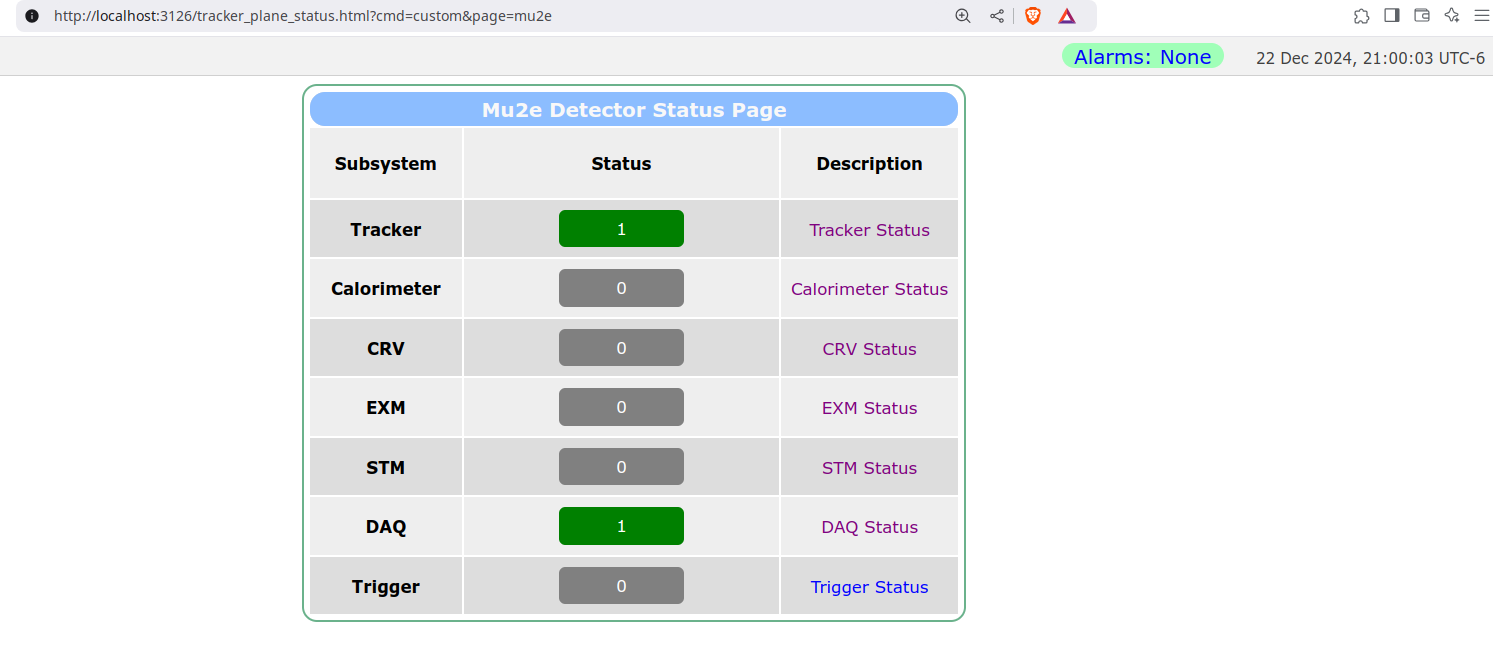
\includegraphics[width=0.95\textwidth]{png/mu2e_status_page}
      }
    };
    % \node [text width=8cm, scale=1.0] at (14.5,0.5) {$\mu_B$, expected background mean};
    % \node [text width=8cm, scale=1.0, rotate={90}] at (1.5,7.5) { $S_{D}$, ``discovery'' signal strength  };
  \end{tikzpicture}
  \caption{
    \label{figure:mu2e_status_page}
    Mu2e status page (prototype)
  }
\end{figure}

State of each enabled configurable element is monitored by a MIDAS frontend.
If a problem is detected, the status of the element is set to a negative
number, which value represents the status code of the problem.

A special configuration frontend propagates the status of the problem up the
configuration tree in ODB. For example, if a problem is detected with one of the
tracker panels, the status box corresponding to the tracker on the top monitoring
page will also become red.

After a problem with the panel is cleared, its status gets set to zero by the
monitoring frontend. The change is propagated up the configuration tree
by the configuration frontend, and the color of the tracker monitoring box
becomes green again.


THe element status box becomes red. 

%%% Local Variables:
%%% mode: latex
%%% TeX-master: t
%%% End:
